\documentclass[journal]{IEEEtran}
\usepackage[a5paper, margin=10mm, onecolumn]{geometry}
%\usepackage{lmodern} % Ensure lmodern is loaded for pdflatex


\setlength{\headheight}{1cm} % Set the height of the header box
\setlength{\headsep}{0mm}     % Set the distance between the header box and the top of the text

\usepackage{gvv-book}
\usepackage{gvv}
\usepackage{cite}
\usepackage{amsmath,amssymb,amsfonts,amsthm}
\usepackage{algorithmic}
\usepackage{graphicx}
\usepackage{textcomp}
\usepackage{xcolor}
\usepackage{txfonts}
\usepackage{listings}
\usepackage{enumitem}
\usepackage{mathtools}
\usepackage{gensymb}
\usepackage{comment}
\usepackage[breaklinks=true]{hyperref}
\usepackage{tkz-euclide} 
\usepackage{listings}
% \usepackage{gvv}                                        
\def\inputGnumericTable{}                                 
\usepackage[latin1]{inputenc}                                
\usepackage{color}                                            
\usepackage{array}                                            
\usepackage{longtable}                                       
\usepackage{calc}                                             
\usepackage{multirow}                                         
\usepackage{hhline}                                           
\usepackage{ifthen}                                           
\usepackage{lscape}
\begin{document}

\bibliographystyle{IEEEtran}
\vspace{3cm}

\title{10.3.2.3.2}
\author{EE24BTECH11033 - Kolluru Suraj}
 \maketitle
% \newpage
% \bigskip
{\let\newpage\relax\maketitle}

\renewcommand{\thefigure}{\theenumi}
\renewcommand{\thetable}{\theenumi}
\setlength{\intextsep}{10pt} % Space between text and floats


\numberwithin{equation}{enumi}
\numberwithin{figure}{enumi}
\renewcommand{\thetable}{\theenumi}


\textbf{Question}:\\
On comparing the ratios $\frac{a_1}{a_2},\frac{b_1}{b_2},and \frac{c_1}{c_2}$, find out whether the following pair of linear equations are consistent, or inconsistent
\begin{align}
    2x-3y=8, 4x-6y=9
\end{align}
\\


\textbf{Theoritical Solution:}
To determine whether the given pair of linear equations is consistent or inconsistent, we compare the ratios $\frac{a_1}{a_2}$, $\frac{b_1}{b_2}$, and $\frac{c_1}{c_2}$, where:
	
	\begin{align}
		a_1x + b_1y = c_1 \quad \text{and} \quad a_2x + b_2y = c_2
	\end{align}
	
	From the equations:
	\begin{align}
		2x - 3y = 8 \quad \text{and} \quad 4x - 6y = 9,
	\end{align}
	we identify:
	\begin{align}
		a_1 = 2, \, b_1 = -3, \, c_1 = 8, \, a_2 = 4, \, b_2 = -6, \, c_2 = 9.
	\end{align}
	
	Now calculate the ratios:
	\begin{align}
		\frac{a_1}{a_2} = 2, \quad \frac{b_1}{b_2} = 2, \quad \frac{c_1}{c_2} = \frac{9}{8}.
	\end{align}
	
	Since:
	\begin{align}
		\frac{a_1}{a_2} = \frac{b_1}{b_2},
	\end{align}
	the given pair of equations is \textbf{inconsistent} and the lines represented by the equations are \textbf{not intersecting}. Therefore, the system of equations has no solution.\\\\
	\textbf{Computational Solution:}
	\newline
	Let us assume the given system of equations are consistent and we will try solving using LU decomposition
	
	Given the system of linear equations:
	\begin{align}
		2x - 3y &= 8, \label{eq1} \\
		4x - 6y &= 9. \label{eq2}
	\end{align}
	
	We rewrite the equations as:
	\begin{align}
		x_1 &= x, \\
		x_2 &= y,
	\end{align}
	giving the system:
	\begin{align}
		2x_1 - 3x_2 &= 8, \label{eq3} \\
		4x_1 - 6x_2 &= 9. \label{eq4}
	\end{align}
	
	\subsection*{Step 1: Convert to Matrix Form}
	We write the system as:
	\begin{align}
		A \mathbf{x} &= \mathbf{b},
	\end{align}
	where:
	\begin{align}
		A &= \begin{bmatrix} 2 & -3 \\ 4 & -6 \end{bmatrix}, \\
		\mathbf{x} &= \begin{bmatrix} x_1 \\ x_2 \end{bmatrix}, \\
		\mathbf{b} &= \begin{bmatrix} 8 \\ 9 \end{bmatrix}.
	\end{align}
	
	\subsection*{Step 2: LU factorization using update equaitons}
    Given a matrix $ \mathbf{A} $ of size $ n \times n $, LU decomposition is performed row by row and column by column. The update equations are as follows:\\
    \textbf{Step-by-Step Procedure:}\\
1. Initialization: 
   - Start by initializing $ \mathbf{L} $ as the identity matrix $ \mathbf{L} = \mathbf{I} $ and $ \mathbf{U} $ as a copy of $ \mathbf{A} $.
   
2. Iterative Update:
   - For each pivot $ k = 1, 2, \ldots, n $:
     - Compute the entries of $ U $ using the first update equation.
     - Compute the entries of $ L $ using the second update equation.
   
3. Result:
   - After completing the iterations, the matrix $ \mathbf{A} $ is decomposed into $ \mathbf{L} \cdot \mathbf{U} $, where $ \mathbf{L} $ is a lower triangular matrix with ones on the diagonal, and $ \mathbf{U} $ is an upper triangular matrix.

    

\subsection*{1. Update for $ U_{k,j} $ (Entries of $ U $)}

For each column $ j \geq k $, the entries of $ U $ in the $ k $-th row are updated as:
\[
U_{k,j} = A_{k,j} - \sum_{m=1}^{k-1} L_{k,m} \cdot U_{m,j}, \quad \text{for } j \geq k.
\]
This equation computes the elements of the upper triangular matrix $ \mathbf{U} $ by eliminating the lower triangular portion of the matrix.

\subsection*{2. Update for $ L_{i,k} $ (Entries of $ L $)}

For each row $ i > k $, the entries of $ L $ in the $ k $-th column are updated as:
\[
L_{i,k} = \frac{1}{U_{k,k}} \left( A_{i,k} - \sum_{m=1}^{k-1} L_{i,m} \cdot U_{m,k} \right), \quad \text{for } i > k.
\]
This equation computes the elements of the lower triangular matrix $ \mathbf{L} $, where each entry in the column is determined by the values in the rows above it.\\
Using a code we get L,U as 
\begin{align}
    L=\begin{bmatrix} 1 & 0 \\ 2 & 1 \end{bmatrix}
    U=\begin{bmatrix} 2 & -3 \\ 0 & 0 \end{bmatrix}
\end{align}

	\subsection*{Step 3: Solve $L\mathbf{y} = \mathbf{b}$ (Forward Substitution)}
	We solve:
	\begin{align}
		L\mathbf{y} = \mathbf{b} \quad \text{or} \quad \begin{bmatrix} 1 & 0 \\ 2 & 1 \end{bmatrix} \begin{bmatrix} y_1 \\ y_2 \end{bmatrix} = \begin{bmatrix} 8 \\ 9 \end{bmatrix}.
	\end{align}
	From the first row:
	\begin{align}
		y_1 &= 8.
	\end{align}
	From the second row:
	\begin{align}
		2 y_1 + y_2 &= 9 \quad \implies \quad 2 \cdot 8 + y_2 = 9 \quad \implies \quad y_2 = -9.
	\end{align}
	
	Thus:
	\begin{align}
		\mathbf{y} &= \begin{bmatrix} 8 \\ -7 \end{bmatrix}.
	\end{align}
	
	\subsection*{Step 4: Solve $U\mathbf{x} = \mathbf{y}$ (Backward Substitution)}
	We solve:
	\begin{align}
		U\mathbf{x} = \mathbf{y} \quad \text{or} \quad \begin{bmatrix} 2 & -3 \\ 0 & 0 \end{bmatrix} \begin{bmatrix} x_1 \\ x_2 \end{bmatrix} = \begin{bmatrix} 8 \\ -7 \end{bmatrix}.
	\end{align}
	From the second row, We get
	\begin{align}
		0=-7
	\end{align}
    which is inappropriate. That means our assumption is wrong
	
	\subsection*{Final Solution}
	Since we are getting inappropriate equations using LU method that means the given system of equations have no solution.\\
    Hence they are inconsistent

\begin{figure}[!ht]
    \centering
    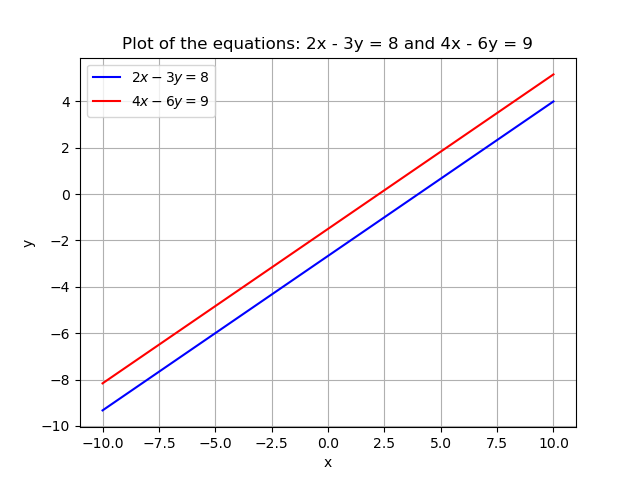
\includegraphics[width=\columnwidth]{figs/Figure_1.png}
    \caption{}
\end{figure}
\end{document}

